% Sandia National Laboratories is a multimission laboratory managed and
% operated by National Technology & Engineering Solutions of Sandia, LLC, a
% wholly owned subsidiary of Honeywell International Inc., for the U.S.
% Department of Energy’s National Nuclear Security Administration under
% contract DE-NA0003525.

% Copyright 2002-2021 National Technology & Engineering Solutions of Sandia,
% LLC (NTESS).

%%-------------------------------------------------------------------------
%% Purpose        : Main LaTeX Xyce Users' Guide
%% Special Notes  : Graphic files (pdf format) work with pdflatex.  To use
%%                  LaTeX, we need to use postscript versions.  Not sure why.
%% Creator        : Scott A. Hutchinson, Computational Sciences, SNL
%% Creation Date  : {05/23/2002}
%%
%%-------------------------------------------------------------------------

\chapter{Simulation Examples with Xyce}
\label{Sim_Examples}

\chapteroverview{Chapter Overview}
{
This chapter provides several simple examples of \Xyce{} usage.
An example circuit is provided for each available analysis type.
\begin{XyceItemize}
\item Section~\ref{Example_Construction}, \emph{Example Circuit Construction}
\item Section~\ref{DC_Sweep}, \emph{DC Sweep Analysis}
\item Section~\ref{Transient_Analysis_Sec}, \emph{Transient Analysis}
\end{XyceItemize}
}

\section{Example Circuit Construction}
\label{Example_Construction}
\index{Example!circuit construction}

This section describes how to use \Xyce{} to create the simple 
diode clipper circuit shown in figure~\ref{Clipper_Schematic}.

\Xyce{} only supports circuit creation via \index{netlist} netlist
editing.  \Xyce{} supports most of the standard netlist entries common
to Berkeley SPICE 3F5\index{SPICE} and Orcad\index{PSpice} PSpice.
For users familiar with PSpice netlists, the \Xyce{} Reference
Guide\ReferenceGuide{} lists the differences between PSpice and \Xyce{}
netlists.  

\subsubsection{Example: diode clipper circuit}

\begin{figure}[H]
\begin{centering}
\shadowbox{
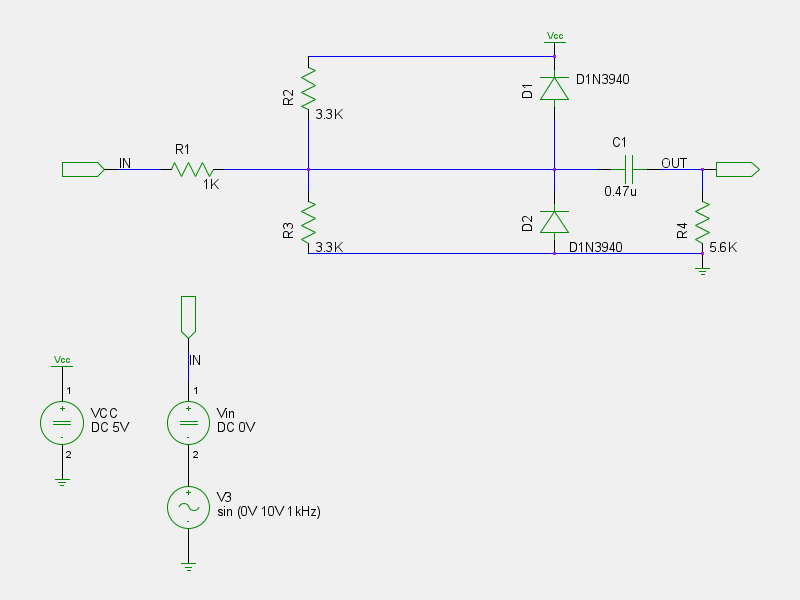
\includegraphics[width=4.5in]{diodeclipper}
}
\caption{Schematic of diode clipper circuit with DC and transient voltage sources.\label{Clipper_Schematic}}
\end{centering}
\end{figure}

Using a plain text editor (e.g., vi, Emacs, Notepad), but not a word processor (e.g., OpenOffice or Microsoft Word), 
create a file containing the netlist of figure ~\ref{Clipper_Netlist_1}. 
For this example, the file is named \texttt{clipper.cir}

The netlist in figure~\ref{Clipper_Netlist_1} illustrates some of the 
syntax of a netlist input file.  Netlists always begin with a 
title line\index{netlist!title} (\emph{e.g.\/} ``\texttt{Diode Clipper Circuit}''), and may 
contain comments\index{netlist!comments} (lines beginning with 
the ``\texttt{*}'' character), devices, and model definitions. Netlists must always end with the ``\texttt{.END}'' statement\index{netlist!\texttt{.END} statement}.

The diode clipper circuit contains two-terminal devices
(diodes, resistors, and capacitors), each of which specifies two
connecting nodes and either a model (for the diode) or a value
(resistance or capacitance).  The netlist of figure~\ref{Clipper_Netlist_1} describes the circuit shown in the schematic of figure~\ref{Clipper_Schematic}

This netlist file is not yet complete and will not run properly using \Xyce{}
(see section~\ref{Running_Xyce} for instructions on running \Xyce{}) as 
it lacks an analysis statement.  This chapter later decribes how to add the appropriate analysis statement and run the diode clipper circuit.

\begin{NetlistFigure}{Diode clipper circuit netlist}{Clipper_Netlist_1}
Diode Clipper Circuit
*
* Voltage Sources
VCC 1 0 5V
VIN 3 0 0V
* Diodes
D1 2 1 D1N3940
D2 0 2 D1N3940
* Resistors
R1 2 3 1K
R2 1 2 3.3K
R3 2 0 3.3K
R4 4 0 5.6K
* Capacitor
C1 2 4 0.47u
*
* GENERIC FUNCTIONAL EQUIVALENT = 1N3940
* TYPE:  DIODE
* SUBTYPE:  RECTIFIER
.MODEL D1N3940 D(
+         IS = 4E-10
+         RS = .105
+          N = 1.48
+         TT = 8E-7
+        CJO = 1.95E-11
+         VJ = .4
+          M = .38
+         EG = 1.36
+        XTI = -8
+         KF = 0
+         AF = 1
+         FC = .9
+         BV = 600
+        IBV = 1E-4)
*
.END
\end{NetlistFigure}

\section{DC Sweep Analysis}
\label{DC_Sweep}
This section includes an example of DC sweep
\index{analysis!DC sweep}\index{DC sweep} analysis using \Xyce{}.  
The DC response of the clipper circuit is obtained by sweeping the DC voltage 
source (\texttt{Vin}) from -10 to 15 volts in one-volt steps.
Chapter~\ref{DC_Analysis} provides more details about DC analysis,  
as does the \Xyce{} Reference 
Guide\ReferenceGuide{}.

\subsubsection{Example: DC sweep analysis}
\index{Example!DC sweep}
To set up and run a DC sweep analysis using the diode clipper circuit:
\begin{enumerate}
\item Open the diode clipper circuit netlist file (\texttt{clipper.cir}) 
using a standard text editor (\emph{e.g.\/} vi, Emacs, Notepad, \emph{etc.\/}).
\index{\texttt{.DC}}
\index{\texttt{.PRINT}!\texttt{DC}}
\item Enter the analysis control statement (as shown in the netlist in figure~\ref{Clipper_Netlist_2}):
\begin{vquote}
.DC VIN -10 15 1
\end{vquote}
\item Enter the output control statement:
\begin{vquote}
.PRINT DC V(3) V(2) V(4)
\end{vquote}
\item Save the netlist file and run \Xyce{} on the circuit. For example, to run
  serial \Xyce{}:
\begin{vquote}
 Xyce clipper.cir
\end{vquote}
\item Open the results file (\texttt{clipper.cir.prn}) and examine (or plot) the 
  output voltages that were calculated for nodes 3 (Vin), 2 and 4 (Out).
  Figure~\ref{Clipper_DCSweep} shows the output plotted as a function of the
  swept variable Vin.
\end{enumerate}

\begin{figure}[H]
\begin{centering}
\shadowbox{
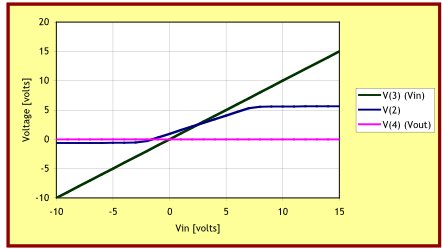
\includegraphics[width=4.5in]{clipper-dcsweep}
}
\caption{DC sweep voltages at Vin, node 2, and Vout\label{Clipper_DCSweep}}
\end{centering}
\end{figure}

\begin{NetlistFigure}{Diode clipper circuit netlist for DC sweep analysis}{Clipper_Netlist_2}
Diode Clipper Circuit with DC sweep analysis statement
*
* Voltage Sources
VCC 1 0 5V
VIN 3 0 0V
* Analysis Command
\color{XyceRed}.DC VIN -10 15 1\color{black}
* Output
\color{XyceRed}.PRINT DC V(3) V(2) V(4)\color{black}
* Diodes
D1 2 1 D1N3940
D2 0 2 D1N3940
* Resistors
R1 2 3 1K
R2 1 2 3.3K
R3 2 0 3.3K
R4 4 0 5.6K
* Capacitor
C1 2 4 0.47u
*
* GENERIC FUNCTIONAL EQUIVALENT = 1N3940
* TYPE:  DIODE
* SUBTYPE:  RECTIFIER
.MODEL D1N3940 D(
+         IS = 4E-10
+         RS = .105
+          N = 1.48
+         TT = 8E-7
+        CJO = 1.95E-11
+         VJ = .4
+          M = .38
+         EG = 1.36
+        XTI = -8
+         KF = 0
+         AF = 1
+         FC = .9
+         BV = 600
+        IBV = 1E-4)
*
.END
\end{NetlistFigure}

\section{Transient Analysis}
\label{Transient_Analysis_Sec}

This section contains an example of transient analysis\index{analysis!transient}
\index{transient analysis} in \Xyce{}.  In this example, the
DC analysis of the diode clipper circuit of the previous section has
been modified so that the input voltage source (\texttt{Vin}) is a
time-dependent sinusoidal input source.  The frequency of \texttt{Vin} is
1 kHz, and has an amplitude of 10 volts.  For more details about transient
analysis see chapter~\ref{Transient_Analysis}, or the \Xyce{} Reference 
Guide\ReferenceGuide{}.

\subsubsection{Example: transient analysis}
\index{Example!transient analysis}

To set up and run a transient analysis using the diode clipper circuit:
\begin{enumerate}
\item Open the diode clipper circuit netlist file file (\texttt{clipper.cir}) 
using a standard text editor (\emph{e.g.\/} VI, Emacs, Notepad, \emph{etc.\/}).
\item Remove DC analysis and output statements if added in the previous example (figure~\ref{Clipper_Netlist_2}).  \index{\texttt{.TRAN}}\index{\texttt{.PRINT}!\texttt{TRAN}}
\item Enter the analysis control (as shown in the netlist in figure~\ref{Clipper_Netlist_3}):
\begin{vquote}
.TRAN 2ns 2ms
\end{vquote}
\item Enter the output control statement:
\begin{vquote}
.PRINT TRAN V(3) V(2) V(4)
\end{vquote}
\item Modify the input voltage source (\texttt{Vin}) to generate the 
sinusoidal input signal:
\begin{vquote}
VIN 3 0 SIN(0V 10V 1kHz)
\end{vquote}
\item 
At this point, the netlist should look similar to the netlist in figure~\ref{Clipper_Netlist_3}.  Save the netlist file and run \Xyce{} on the circuit.  For example, to run serial \Xyce{}:
\begin{vquote}
 Xyce clipper.cir
\end{vquote}
\item Open the results file and examine (or plot) the output voltages for 
nodes 3 (\texttt{Vin}), 2, and 4 (\texttt{Out}).  The plot in
  figure~\ref{Clipper_Trans} shows the output plotted as a function of time.
\end{enumerate}
Figure~\ref{Clipper_Netlist_3} shows the modified netlist and figure~\ref{Clipper_Trans} shows the
corresponding results.

\begin{NetlistFigure}{Diode clipper circuit netlist for transient analysis}{Clipper_Netlist_3}
Diode clipper circuit with transient analysis statement
*
* Voltage Sources
VCC 1 0 5V
\color{XyceRed}VIN 3 0 SIN(0V 10V 1kHz)\color{black}
* Analysis Command
\color{XyceRed}.TRAN 2ns 2ms\color{black}
* Output
\color{XyceRed}.PRINT TRAN V(3) V(2) V(4)\color{black}
* Diodes
D1 2 1 D1N3940
D2 0 2 D1N3940
* Resistors
R1 2 3 1K
R2 1 2 3.3K
R3 2 0 3.3K
R4 4 0 5.6K
* Capacitor
C1 2 4 0.47u
*
* GENERIC FUNCTIONAL EQUIVALENT = 1N3940
* TYPE:  DIODE
* SUBTYPE:  RECTIFIER
.MODEL D1N3940 D(
+         IS = 4E-10
+         RS = .105
+          N = 1.48
+         TT = 8E-7
+        CJO = 1.95E-11
+         VJ = .4
+          M = .38
+         EG = 1.36
+        XTI = -8
+         KF = 0
+         AF = 1
+         FC = .9
+         BV = 600
+        IBV = 1E-4)
*
.END

\end{NetlistFigure}

\begin{figure}[H]
  \begin{centering}
    \shadowbox{
      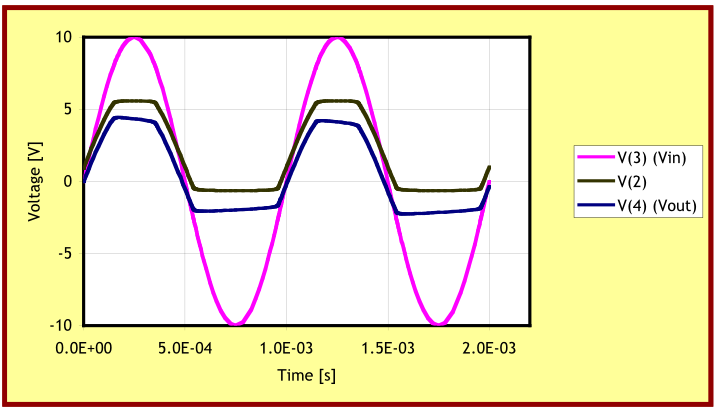
\includegraphics[width=4.5in]{clipper-trans}
    }
    \caption{Sinusoidal input signal and clipped outputs\label{Clipper_Trans}}
  \end{centering}
\end{figure}

%%% Local Variables:
%%% mode: latex
%%% End:
% END of Xyce_UG_ch03.tex ************
